\documentclass{beamer}
\usepackage[utf8]{inputenc}

%% ADDITIONAL NICOLÁS
\usepackage{ragged2e}
\usepackage{amssymb}
\usefonttheme{serif}
%% ADDITIONAL NICOLÁS



\usetheme{Madrid}
\usecolortheme{default}

%------------------------------------------------------------
%This block of code defines the information to appear in the
%Title page
\title[Weekly Reports] %optional
{PhD in Energy and Mineral Engineering at PSU}

\subtitle{Nicolás's Research - Reports}

\author[Nicolás Bueno] % (optional)
{Nicolás Bueno\inst{1} \and Advisor: Dr. Ayala\inst{1}}

\institute[EME] % (optional)
{
	\inst{1}%
	Department of Energy and Mineral Engineering\\
	Penn State University\\
	
\includegraphics[height=1cm]{pics/PSU_EMS.png}
}

\date[Fall 2021] % (optional)
{}

%\logo{
\includegraphics[height=1cm]{pics/PSU_EMS.png}}

%End of title page configuration block
%------------------------------------------------------------



%------------------------------------------------------------
%The next block of commands puts the table of contents at the 
%beginning of each section and highlights the current section:

\AtBeginSection[]
{
	\begin{frame}
		\frametitle{Table of Contents}
		\tableofcontents[currentsection]
	\end{frame}
}
%------------------------------------------------------------


\begin{document}
	
	%The next statement creates the title page.
	\frame{\titlepage}
	
	%---------------------------------------------------------
	%This block of code is for the table of contents after
	%the title page
	\begin{frame}
		\frametitle{Table of Contents}
		\tableofcontents
	\end{frame}
	%---------------------------------------------------------
	
	\justifying
	\section{Fall 2021}
	
	\subsection{Report Sep 16 - 2021}
	\begin{frame}
		\textbf{Report Sep 16 - 2021}\\~\\
		Main discussion points:
		\begin{itemize}
			\item Generalities
			\item Cheng's paper
			\item Dr. Yashar and Miscible code
			\item Plausible models for thermodynamic coupling
		\end{itemize}
	\end{frame}
	
	\begin{frame}
		\frametitle{Generalities}
		Trip to New York next week (Friday)\\~\\
		Paper affiliation for paper recently accepted (yesterday)\\~\\
		Format of future presentations and meeting setup
	\end{frame}
	
	\begin{frame}
		\frametitle{Cheng's paper}
		I was running some codes (those with more than 1 time step). They are now stored in my OneDrive and my laptop. What I found:
		\begin{itemize}
			\item<1-> \alert{Different versions} of the same code
			\item<2-> They compile and run correctly (the tested ones). Visualization adapted from the code I developed for William's cases. \alert{Run cases}: 
			\begin{itemize}
				\item<2-> Droplet impacting surface (MCMP and IMM?)
				\item<2-> Oscillating droplet
				\item<2-> Rotating droplet
				\item<2-> Surface wave
			\end{itemize}
			\item<3-> DRY
		\end{itemize}
	\end{frame}
	
	\begin{frame}
		\frametitle{Cheng's paper}
		With these results we are able to:
		\begin{itemize}
			\item Decide which dynamic \alert{metrics} will be tracked to validate/analyze/compare
			\item Play around with some parameters to see how they impact the dynamic metrics
		\end{itemize}
	\end{frame}

	\begin{frame}
		\frametitle{Cheng's paper}
		
		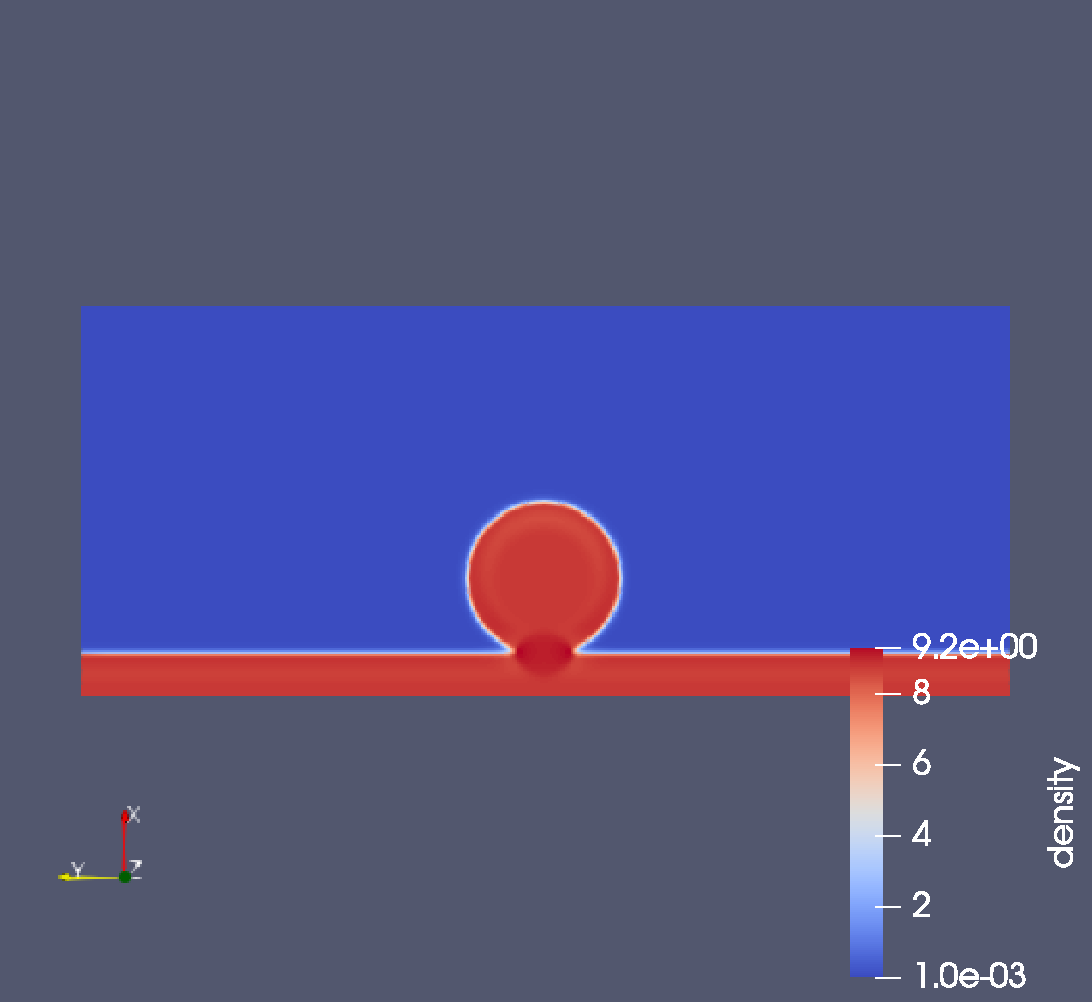
\includegraphics[scale=0.2]{pics/impactingDroplet.pdf}
		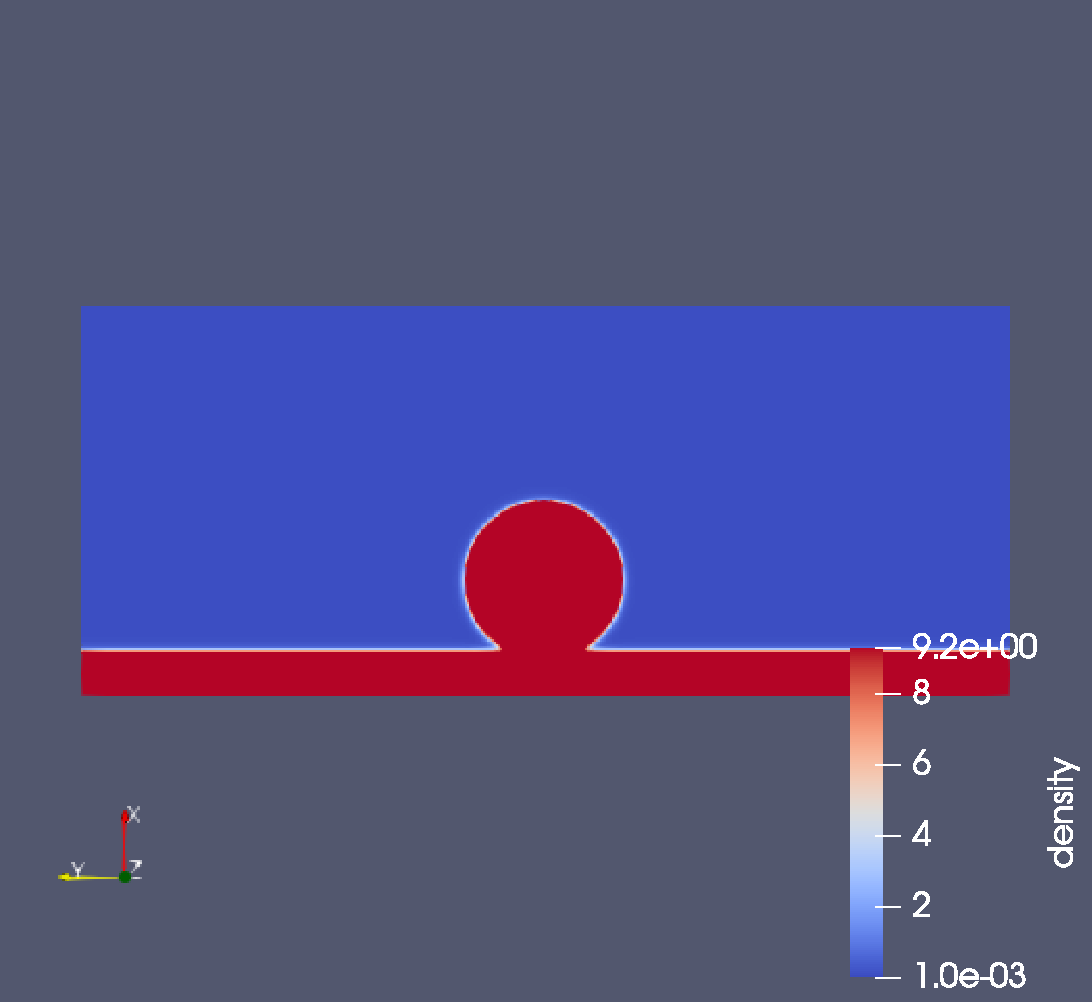
\includegraphics[scale=0.2]{pics/impactingDropletMCMP.pdf}\\
		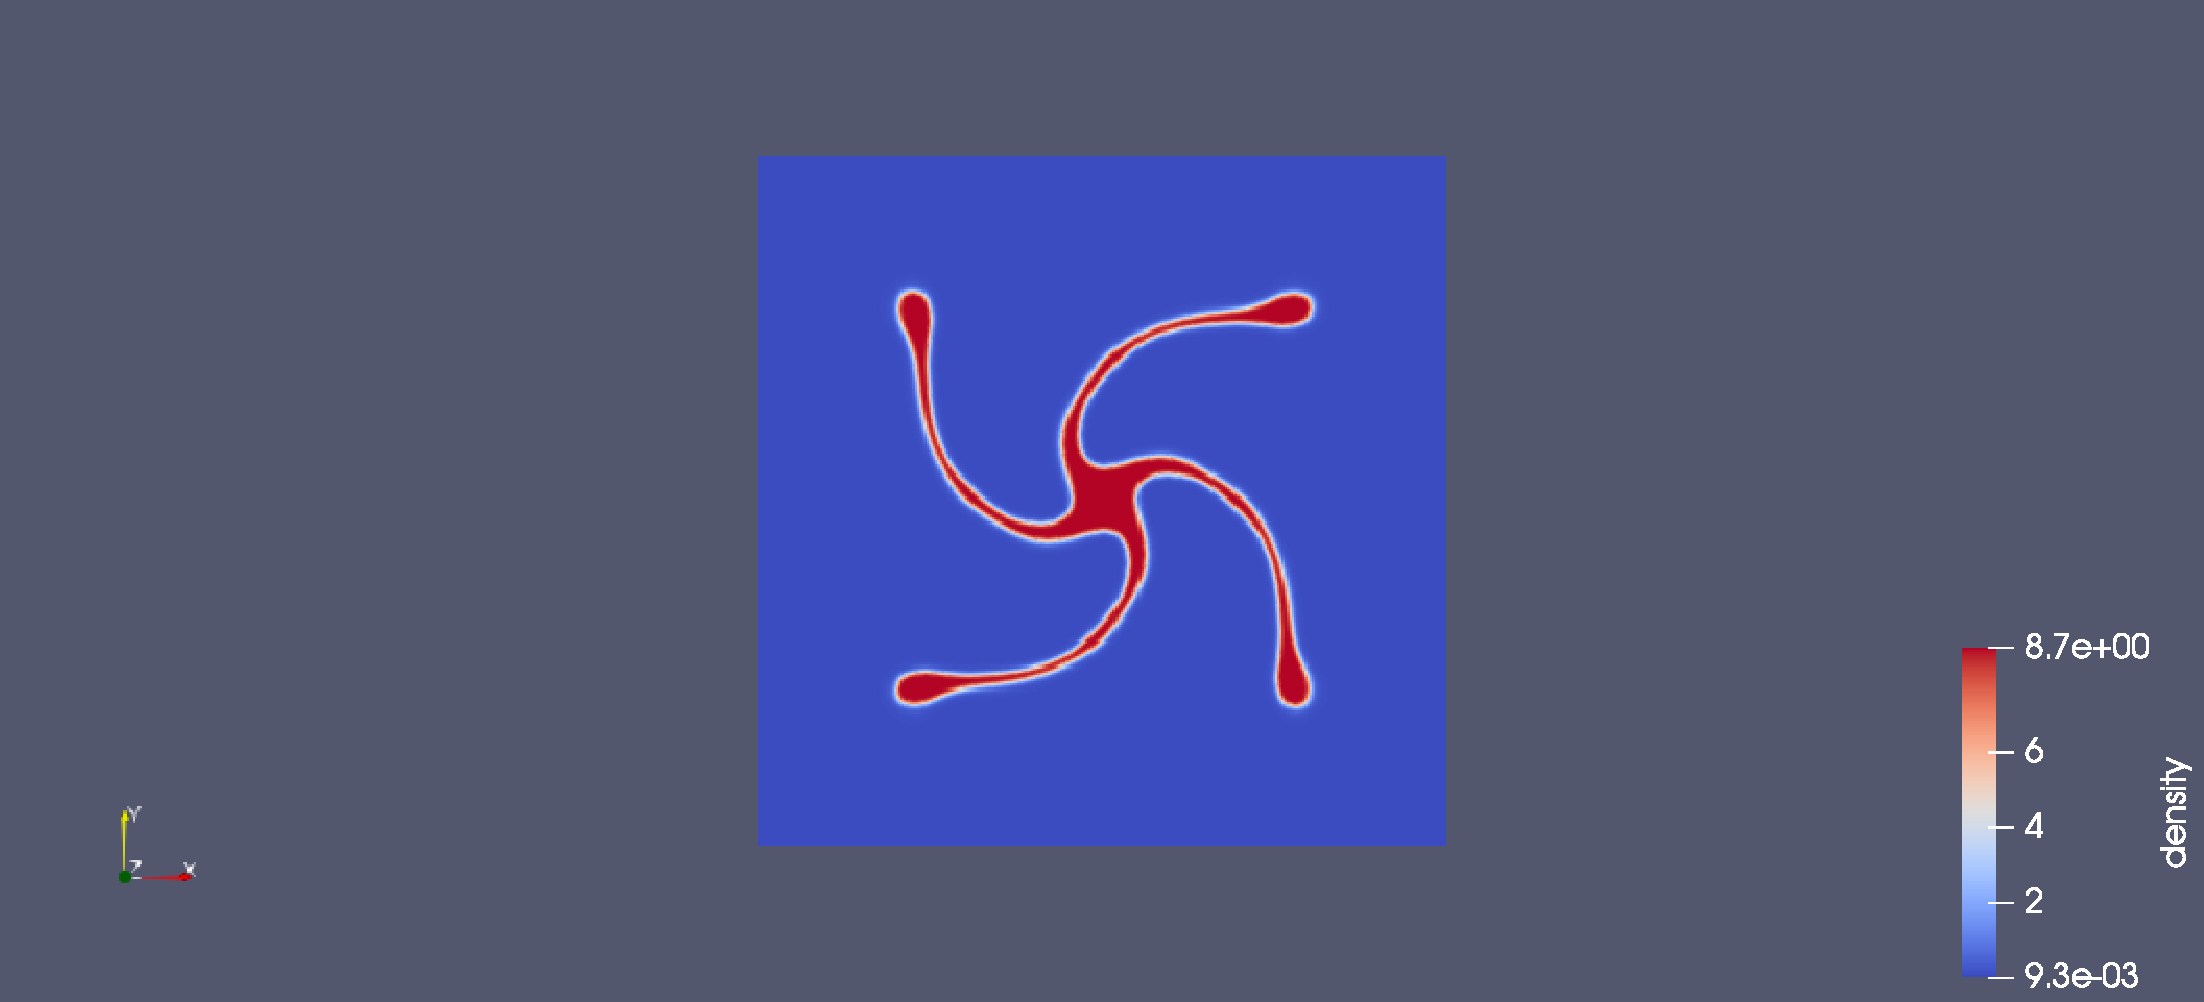
\includegraphics[scale=0.2]{pics/rotatingDroplet.pdf}
	\end{frame}

	\begin{frame}
		\frametitle{Dr. Yashar and Miscible Code}
		\begin{columns}[T]
			
			\column{0.4\textwidth}
			\justifying
			The new code already contains: scaling,	two-phase equilibrium, initialization of parameters. Next step:\\ DF initialization.
			
			\column{0.4\textwidth}
			Before comparing programming languages, state its requirements:
			\begin{itemize}
				\item Parallelization. Garbage collector. 
				\item 3D simulation (large memory usage)
				\item Maintainable and easy to couple with other tools
			\end{itemize}
		\end{columns}
	\end{frame}

	\begin{frame}
		\frametitle{Plausible models for thermodynamic coupling}
		\centering
		\textbf{Comprehensive comparison of pore-scale models for multiphase flow in porous media}\\~\\
		\justifying
		Paper comparing bench-marking pore-scale methods against experimental data, varying $C_a$ and wettability.
		
		\begin{itemize}
			\item LBM higher resolution ($\sim$ 14 $\mu$m/lattice)
			\item Simulation metrics: fractal dimension ($D_f$), finger width ($W_f$)
			\item LBM captures thin films and corner flow (3D effect). Computationally costly.
		\end{itemize}
		\begin{block}{Phase Field (Quasi 3D method)}
			Capture incomplete displacement (film flow) but not corner flow
		\end{block}
		
	\end{frame}
	
	\begin{frame}
		\centering
		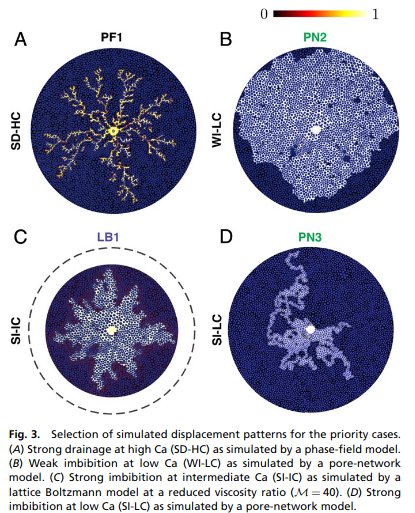
\includegraphics[scale=0.4]{pics/paperScenarios.png}
	\end{frame}
	
	\begin{frame}
		Additional comments on phase field and LBM
		\begin{itemize}
			\item LBM requires $\sim$ 160 million cells. Limited by viscosity ratio $M$ and in the limit of thin films
			\item 3D simulation is recommended
			\item Phase field looks promising to capture 3D effects with reduced computational cost, at high $M$, depending on regime
			\item All of them capture viscous fingering in some degree
			\item Many-pore scale is the only way to capture flow dynamics
		\end{itemize}
	\end{frame}

	\begin{frame}
		\frametitle{Comments...}
		\begin{itemize}
			\item Shared Google Drive
			\item Keep going fast with the new code
			\item Read last Cheng's paper and see how the simulations there can be connected with the needs in the second one
			\item Analytical solutions as a validation after comparing with Cheng's code
			\item Be ready for programming language discussion
			\item How different LBM models are formulated?
			\item Study in deep a phase field formulation to understand what it has inside
			\item PhD position
		\end{itemize}
		
	\end{frame}
	%---------------------------------------------------------
	%---------------------------------------------------------
	
	\subsection{Report Sep 30 - 2021}
	\justifying
		\begin{frame}
			\textbf{Report Sep 30 - 2021}\\~\\
			Main discussion points:
			\begin{itemize}
				\item Generalities
				\item Code state
				\item PhD position
				\item Communications with Cheng and Dr. Mehmani
			\end{itemize}
		\end{frame}
		
		\begin{frame}{Generalities}
			\begin{itemize}
				\item<1-> Courses: 
				\begin{itemize}
					\item Programming: Gained C++ proficiency: classes, pointers, functions (...). Weekly programming homework and quizzes. 
					\item Data mining: Exploring more classification algorithms, their cost functions, and implications. First project submitted on Sunday.
					\item CHE 524: Entropy functional and probabilities. Final exam: Dec 13.
					\item AERSP 508: Solving analytically flow for inviscid-incompressible flow.
				\end{itemize}

				\item<2-> Came on Monday from New Jersey. Everything good
				\item<3-> Paper about LBM for aneurysm \href{https://www.mdpi.com/2311-5521/6/10/338/htm}{\textcolor{blue}{(link)}}
				\item<4-> Worked for SIATA on Tuesday
			\end{itemize}
		\end{frame}
		
		\begin{frame}{Code state}
			EoS partially validated.\\ Compressibility factor highly deviated from a particular pressure/composition combination.\\ Changed functions to be vectorized
			\begin{block}{Remark}
				I didn't advance as expected (putting attention on other PhD tasks) but is ongoing. As I am comparing codes, the double screen will be a key point to me.
			\end{block}
			
			
		\end{frame}
		
		\begin{frame}{Multiple phases in a single lattice}
			Do you agree that in a single lattice, multiple phases may coexist in a particular time step?\\~\\ \pause
			If no, how to justify that a particular combination of composition and total density (or pressure) always honors thermodynamics in a stable phase.\\~\\ \pause
			If yes, shouldn't the model compute a split factor for each phase (as force is computed for phases) and then sum up the force for each component in each phase?
		\end{frame}
		
		\begin{frame}{PhD position}
			Hillmert Solano and Juliana Rueda
		\end{frame}
	
		\begin{frame}{Communications with Cheng and Dr. Mehmani}
			\begin{columns}[T]
				\column{0.4\textwidth}
				\justifying
				To Cheng's email:\\
				\alert{Check Outlook}
				
				\column{0.4\textwidth}
				Dr. Mehmani email:
				\begin{itemize}
					\item 1-2 slides with governing equations. 
					\item Simulation results
					\item Open discussion (methods, tools,...)
				\end{itemize}
			\end{columns}
		\end{frame}
	
		\begin{frame}
			\frametitle{Others}
			\begin{itemize}
				\item Google Drive ready
				\item Screen received and waiting for the workstation
				\item Plan to incorporate Inkscape to these presentations
			\end{itemize}
		\end{frame}
	
		\begin{frame}
			\frametitle{Actions}
			\begin{itemize}
				\item Advance in the code and prepare presentation with governing equations for Dr. Mehmani
				\item Send Fluid mechanics book
				
				\item Week ideas: validation cases can be found in the Paper 005.
			\end{itemize}
		\end{frame}
		%---------------------------------------------------------
		%---------------------------------------------------------
		
		
		\subsection{Meeting Nicolas - Dr. Mehmani - 2021}
		\justifying
		\begin{frame}
			\textbf{Meeting Nicolas - Dr. Mehmani - 2021}\\~\\
			Main discussion points:
			\begin{itemize}
				\item Governing equations
				\item Results with current model
				\item State of new version
			\end{itemize}
		\end{frame}
		
		
		\begin{frame}
			\frametitle{Governing equations}
			
			The Lattice Boltzmann Method is based on kinetic theory, that states:
			
			\begin{equation}\label{eq:LBPDE}
			\underbrace{\frac{\partial f_i(x,t)}{\partial t} + \mathbf{c}_i \frac{\partial f_i(x,t)}{\partial x}}_{\text{Streaming - DF Advection}} = \underbrace{\mathbf{\Omega}}_{\text{Collision}} 
			\end{equation}
			
			What in its discretized form\footnote{Going from \ref{eq:LBPDE} to \ref{eq:LBE}, what about spatial derivative?} becomes:
			\begin{equation}\label{eq:LBE}
				f_i(x+ \mathbf{c}_i \Delta t, t+\Delta t) - f_i(x, t) = - \mathbf{M}^{-1} \mathbf{S} [\mathbf{m}(x,t) - \mathbf{m}^{\text{eq}}]  + \hat{F}_i
			\end{equation}
			where $\mathbf{m}$ are vectors of moments, $\mathbf{S}$ is a relaxation diagonal matrix, and $\mathbf{M}$ is a fixed matrix depending on DnQm. $ \mathbf{m}^{\text{eq}} = f(f_i^{\text{eq}}, \mathbf{F})$.
		\end{frame}
		
		
		\begin{frame}
			\frametitle{Macroscopic variables}
			Density and velocity are computed as follows:
			\begin{equation}
				\rho = \sum_i f_i \, \, \, \, \, \, \, \,  \mathbf{u} = \sum_i \mathbf{c}_i f_i
			\end{equation}
			Two important constitutive equations:
			\begin{equation*}
				f_i^{\text{eq}} = \rho \omega_i \left[ 1 + \frac{\vec{u}\cdot \vec{\mathbf{c}_i}}{c^2_s} + \frac{(\vec{u}\cdot \vec{\mathbf{c}_i})^2}{2c^4_s}-  \frac{\vec{u}\cdot \vec{u}}{2c^2_s} \right]
			\end{equation*}
			
			\begin{equation*}
			\hat{F}_i = \frac{\mathbf{F}}{\rho} \frac{\vec{u} - \vec{\mathbf{c}_i}}{c^2_s} f_i^{\text{eq}}  
			\end{equation*}
			
			where $\mathbf{F}$ is defined in the multiphase problem, as the Shan Cheng force:
			\begin{equation}
				\mathbf{F} = -G \psi(x) \sum_i \omega_i \psi(x+\mathbf{c}_i \delta t) \mathbf{c}_i \, \, \, \, \, \psi := \sqrt{\frac{2(P^{\text{\tiny EoS}}-c_s^2\rho)}{G \delta t c_s^2}}
			\end{equation}
		\end{frame}
		\begin{frame}
			\frametitle{Droplet impacting on a surface - Immiscible}
			\begin{figure}
				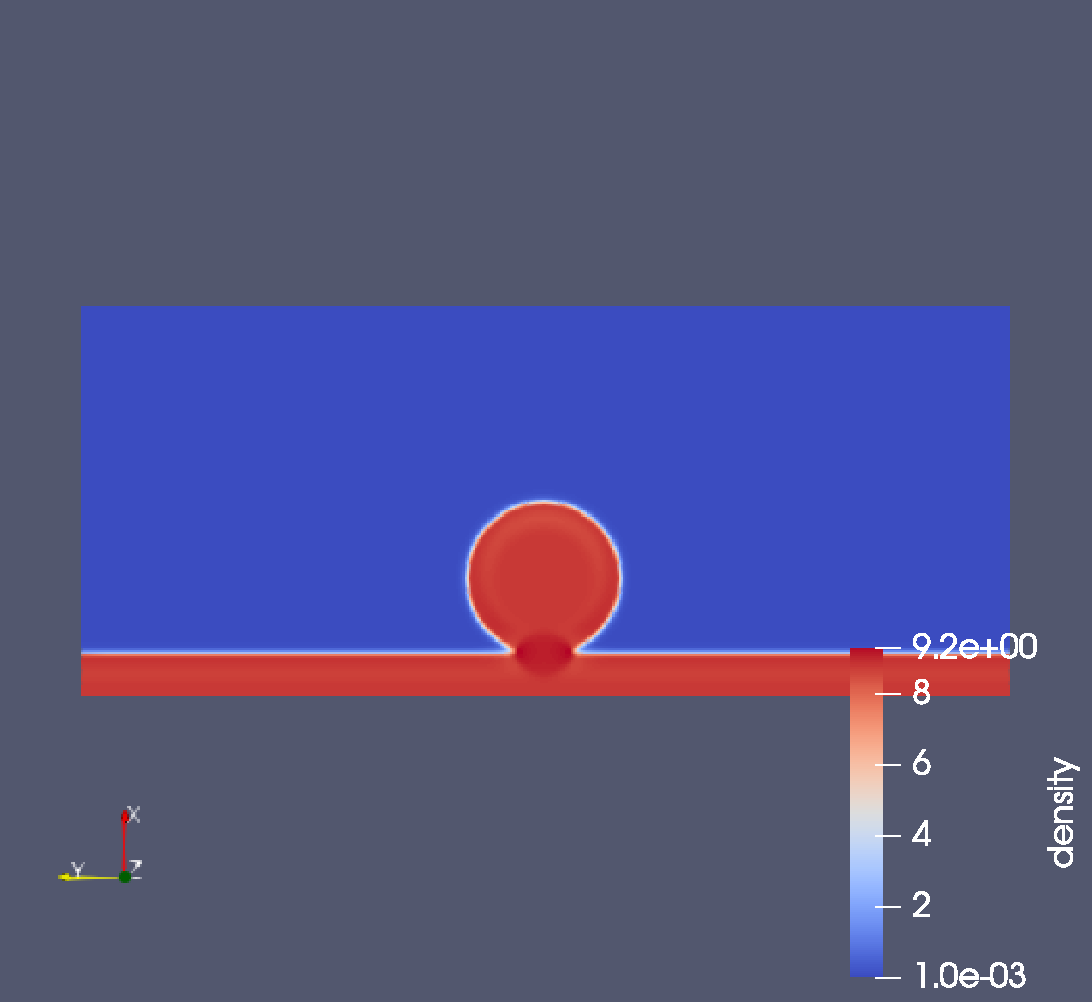
\includegraphics[scale=0.4]{pics/impactingDroplet.pdf}
			\end{figure}
		\end{frame}
		
		\begin{frame}
			\frametitle{Droplet impacting on a surface - Miscible}
			\begin{figure}
				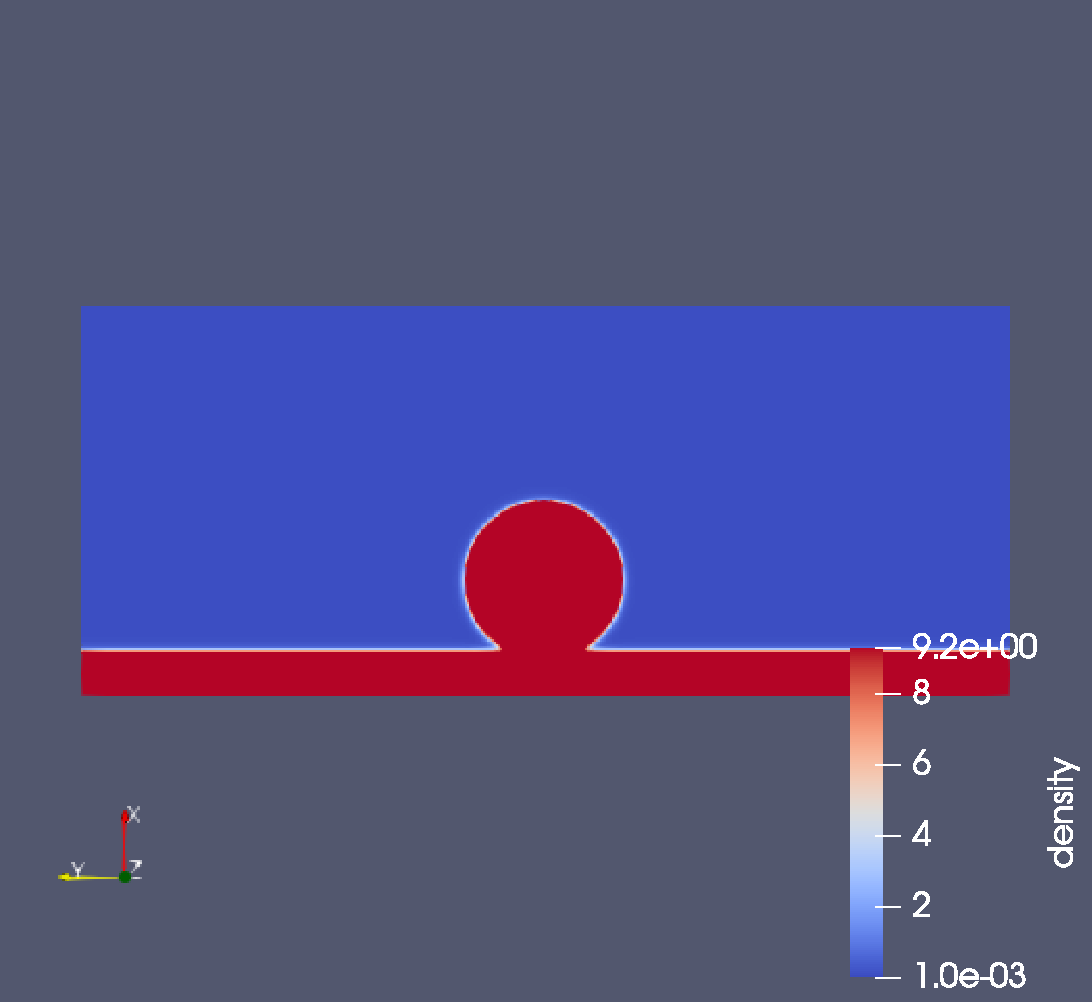
\includegraphics[scale=0.4]{pics/impactingDropletMCMP.pdf}
			\end{figure}
		\end{frame}
		
		\begin{frame}
			\frametitle{Rotating droplet}
			\begin{figure}
				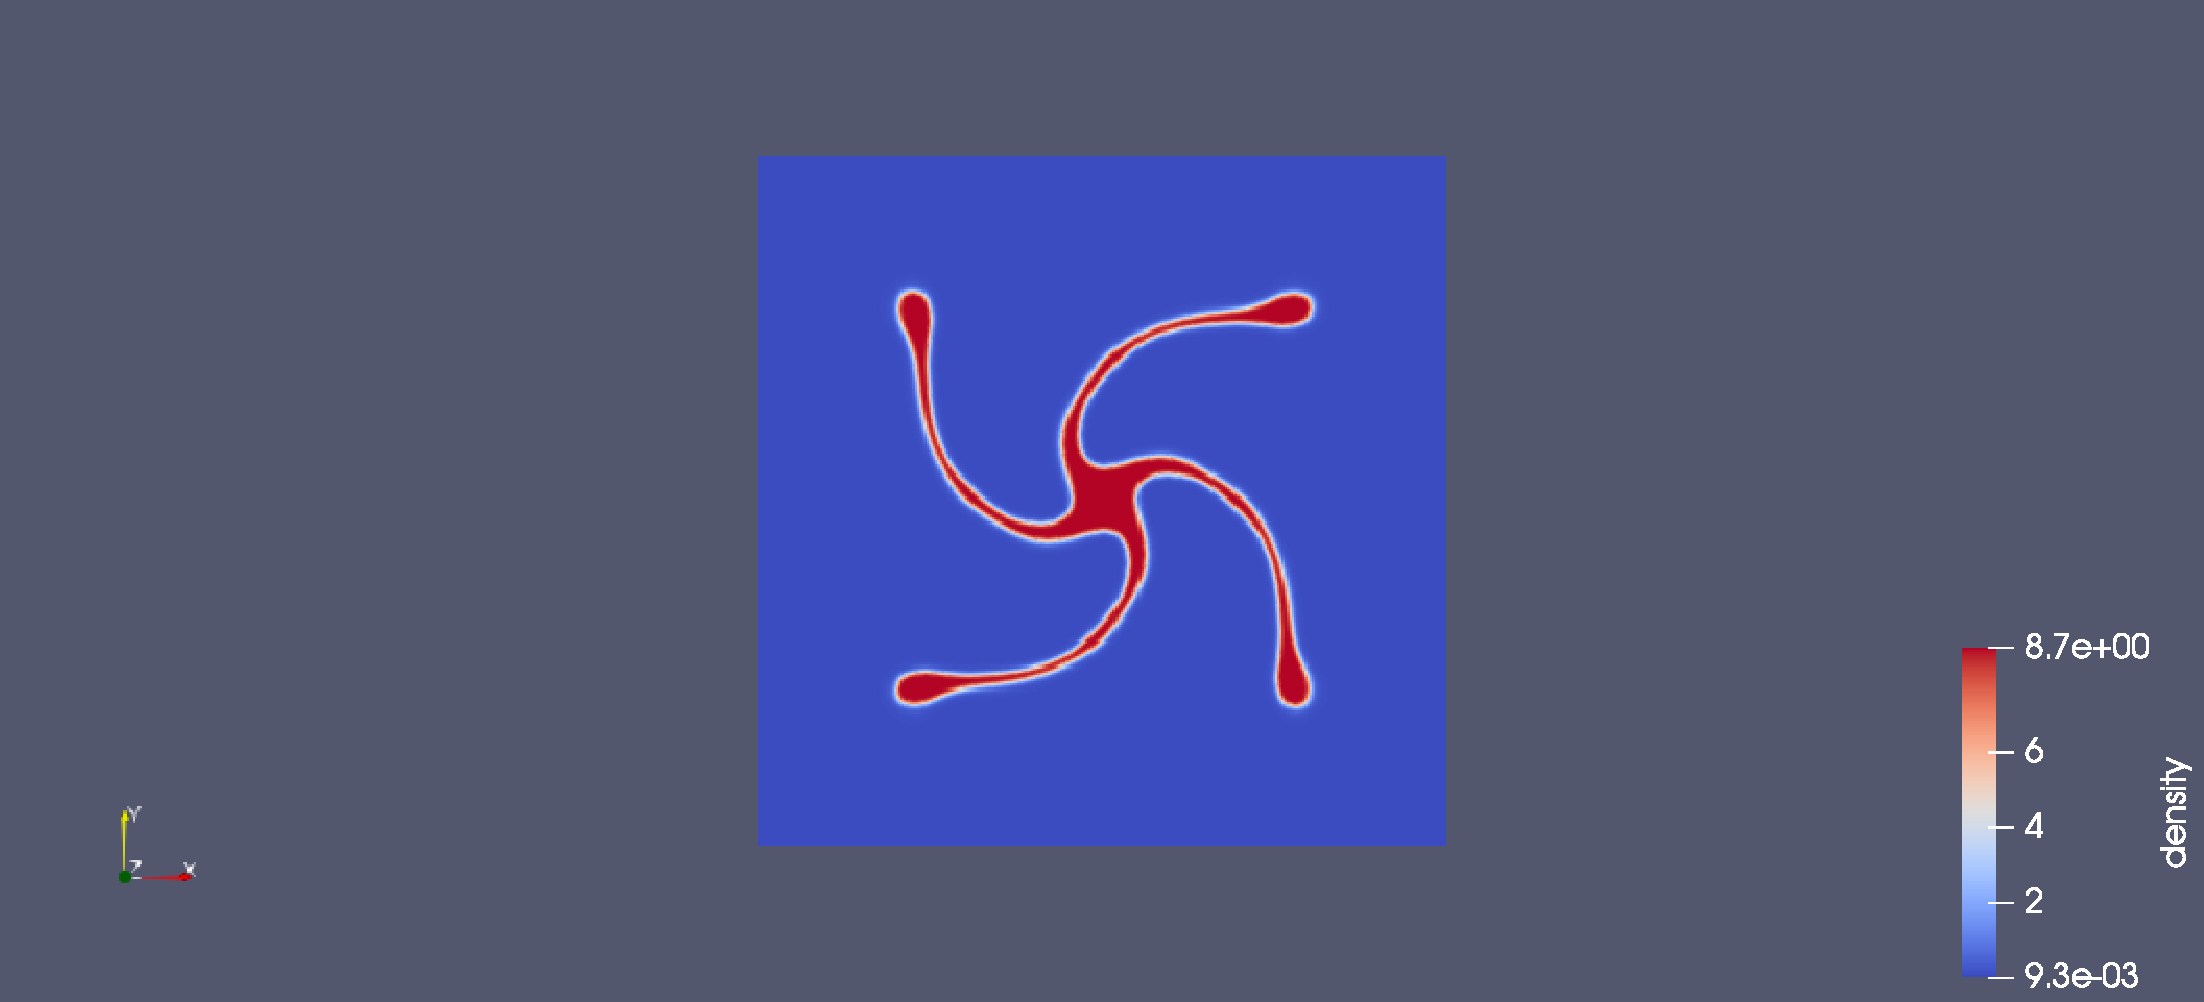
\includegraphics[scale=0.3]{pics/rotatingDroplet.pdf}
			\end{figure}
		\end{frame}
		
	
		\begin{frame}
			\frametitle{State of new version}
			\begin{itemize}
				\item Object oriented Fortran code
				\item VTK-format printing to visualize with Paraview
				\item EoS completely detached from LBM: using inheritance for classes\footnote{Developed in international system of units}
				\item Tools being used:
				\begin{itemize}
					\item Visual Studio Code as interface. Compiler: gfortran
					\item Visualization: ParaView. Not using VTK libraries yet
					\item Makefiles. Not CMake yet
				\end{itemize}
			\end{itemize}
			\begin{alertblock}{Philosophy}
				Decouple physical concepts from numerical concepts\\
				Flexible code for future implementations
			\end{alertblock}
		\end{frame}
		
		\begin{frame}
			\frametitle{Questions}
			Clarification. I am attempting to finish the code for 3 reasons: unify versions and capabilities, having fun, and: materialize on my code the possible PhD projects. Should I attempt to take advantage of this stage to program in parallel other methods?
			
			My concerns: should I start now in C++? Should I start with OF as well? What about other modern/promising methods? Will this be my entry point to the academia?
		\end{frame}
		
		\begin{frame}
			\frametitle{Questions}
			\begin{itemize}
				\item If you were to start your PhD again, which topic/method/language/project would you start? 
				\item Pore-scale phenomenology, most relevant set of equations and ideal solutions for pore-scale modeling, origin of Young Laplace equation, assumptions, etc...
			\end{itemize}
		\end{frame}
		
		\begin{frame}
			End...
		\end{frame}
	
		\begin{frame}{Actions}
			\begin{itemize}
				\item Is F representing other possible forces? van der Waals, Coulomb, walls. \item Write down here the derivation on the board.
				\item Yashar has a code for level-set and volume-of-fluid which to contrast with if I want to develop those methods by myself.
				\item Get used to those methods, derivations, force definitions and the core of the solution: coloring function
				\item C++ with an automatic differentiation library? Can I connect it to Python library? This may reduce my coding time by a factor of 4!
				\item Memorize advection equation, stress tensor definition, forces... 
				\item Concise but better detailed LBM explanation. How surface tension force arises in LBM? Also, do not show results if there is not a good reason to show them (happened with ready simulations).
				
			\end{itemize}
		\end{frame}
		%---------------------------------------------------------
		%---------------------------------------------------------
		
		\subsection{Report Oct 7 - 2021}
		\justifying
		\begin{frame}
			\textbf{Report Oct 7 - 2021}\\~\\
			Main discussion points:
			\begin{itemize}
				\item Generalities
				\item Code state
			\end{itemize}
		\end{frame}
			
		\begin{frame}{Generalities}
			\begin{itemize}
				\item<1-> New machine status: 
				\begin{itemize}
					\item Working as expected (really well!)
					\item Need to contact John: installation in limited/storage disk (remote)
					\item Need permissions to set up my Google Drive account
					\item Compilers working well! gfortran and g++
				\end{itemize}
				\item<2-> Question: without having to solve two distribution functions per component, can we solve an isochoric version of the EoS for every node? 
			\end{itemize}
		\end{frame}
		
		\begin{frame}{Code state}
			Show code status and results connected to ParaView.
		\end{frame}
		
		\begin{frame}{Comparison of EoS Results}
			
			
			\begin{table}
				\centering
				\begin{tabular}{cccc}
					Variable & Old & New & Decimal Pos. Diff\\
					\hline
					$P$ scale & 2987.2198 & 2987.2707 & 2\\
					$T$ scale & 1146.9220 & 1146.9129 & 2\\
					$a_1$ scale & 0.18367 & 0.18367 & 14\\
					$b_2$ scale & 0.28177 & 0.28177 & 6\\
					$Z$ liquid & 0.438672 & 0.438672 & 9\\
					$Z$ gas & 0.59443 & 0.59443 & 10					
				\end{tabular}
				\label{table-P1i}
				\caption{The results related to a thermodynamic conditions, were evaluated at 1888.2 psi}
			\end{table}
		\end{frame}
	
		%\begin{frame}{Code state} 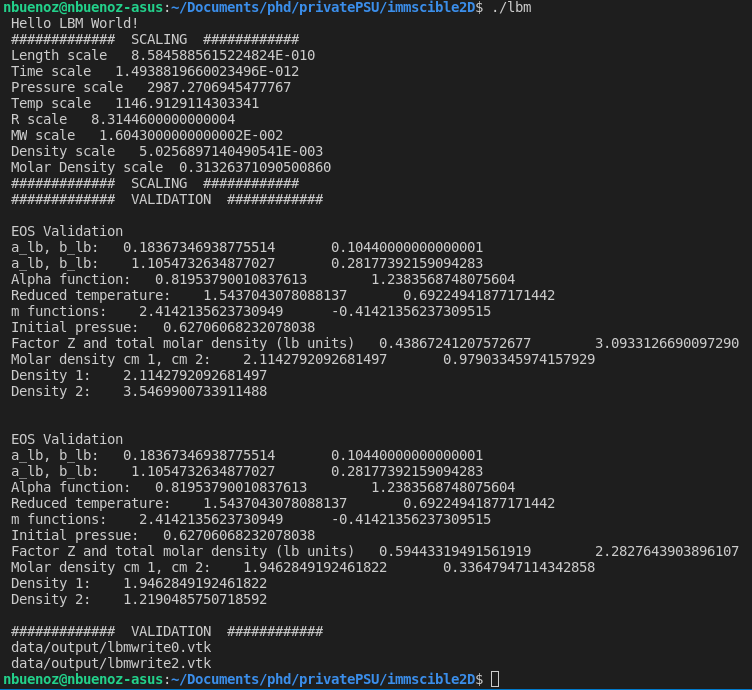
\includegraphics[width=0.4\textwidth]{pics/eosNew.png} 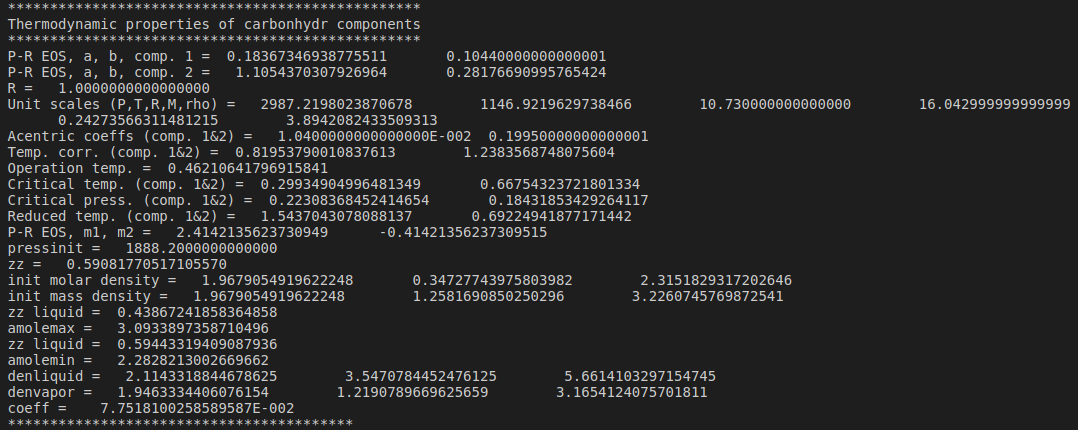
\includegraphics[width=0.6\textwidth]{pics/eosOld.png} \end{frame}
		
		\begin{frame}{Validation of the code}
			\justifying
			\begin{itemize}
				\item Cheng's version and William's version
				\item Closed tube to see linearity of capillary pressure and contact angle
				\item Evaporation from a channel (analytical solution)
			\end{itemize}
		\end{frame}
	
		\begin{frame}{How to keep the momentum?}
			Should I...
			\begin{itemize}
				\item Start visualizing a particular method as potential for us? How to approach to it?
				\item Accelerate any process in which I am being slow?
			\end{itemize}
		
			CVs: Hillmert and Felipe. Upgrading paper.
		\end{frame}
	%---------------------------------------------------------
	%---------------------------------------------------------
	
	\subsection{Report Oct 14 - 2021}
	\justifying
	\begin{frame}
		\textbf{Report Oct 14 - 2021}\\~\\
		Main discussion points:
		\begin{itemize}
			\item Courses
			\item Review the last week missing points
			\item Code state
		\end{itemize}
	\end{frame}
	
	\begin{frame}{Courses}
		
	\end{frame}
	
	\begin{frame}{Code state}
	\begin{itemize}
		\item I ran the fractured porous media simulation from William. I plan to compare against this case first.
		\item New implementations: pseudo potential calculation, Shan-Cheng force, and collision (50\%).
	\end{itemize}
	\end{frame}

	\begin{frame}{Actions}
		\begin{itemize}
			\item Validate first single component multiphase and multicomponent multiphase immiscible cases.
			\item Review the mathematical form of those equations more than implementation.
			\item Keep doing best effort with the courses
		\end{itemize}
	\end{frame}

%---------------------------------------------------------
%---------------------------------------------------------



	%---------------------------------------------------------
	%---------------------------------------------------------
	%---------------------------------------------------------
	%---------------------------------------------------------
	%---------------------------------------------------------
	%---------------------------------------------------------
	%---------------------------------------------------------
	%---------------------------------------------------------
	%---------------------------------------------------------
	
	
	
	\section*{Useful frame options}
	%---------------------------------------------------------
	\begin{frame}
		\textbf{Report XXX XX - 202X}\\~\\
		Main discussion points:
		\begin{itemize}
			\item Topic 1
			\item Topic 2
		\end{itemize}
	\end{frame}
	%---------------------------------------------------------

	%---------------------------------------------------------
	\begin{frame}
	\end{frame}
	%---------------------------------------------------------
	%---------------------------------------------------------
	\begin{frame}
	\end{frame}
	%---------------------------------------------------------
	%---------------------------------------------------------
	\begin{frame}
	\end{frame}
	%---------------------------------------------------------
		%---------------------------------------------------------
	%Changing visivility of the text
	\begin{frame}
		\frametitle{Sample frame title}
		This is a text in second frame. For the sake of showing an example.
		
		\begin{itemize}
			\item<1-> Text visible on slide 1
			\item<2-> Text visible on slide 2
			\item<3> Text visible on slides 3
			\item<4-> Text visible on slide 4
		\end{itemize}
	\end{frame}
	
	%---------------------------------------------------------
	
	
	%---------------------------------------------------------
	%Example of the \pause command
	\begin{frame}
		In this slide \pause
		
		the text will be partially visible \pause
		
		And finally everything will be there
	\end{frame}
	%---------------------------------------------------------
	
	%---------------------------------------------------------
	%Highlighting text
	\begin{frame}
		\frametitle{Sample frame title}
		
		In this slide, some important text will be
		\alert{highlighted} because it's important.
		Please, don't abuse it.
		
		\begin{block}{Remark}
			Sample text
		\end{block}
		
		\begin{alertblock}{Important theorem}
			Sample text in red box
		\end{alertblock}
		
		\begin{examples}
			Sample text in green box. The title of the block is ``Examples".
		\end{examples}
	\end{frame}
	%---------------------------------------------------------
	
	
	%---------------------------------------------------------
	%Two columns
	\begin{frame}
		\frametitle{Two-column slide}
		
		\begin{columns}
			
			\column{0.5\textwidth}
			This is a text in first column.
			$$E=mc^2$$
			\begin{itemize}
				\item First item
				\item Second item
			\end{itemize}
			
			\column{0.5\textwidth}
			This text will be in the second column
			and on a second tought this is a nice looking
			layout in some cases.
		\end{columns}
	\end{frame}
	%---------------------------------------------------------
	
	
\end{document}